% Options for packages loaded elsewhere
\PassOptionsToPackage{unicode}{hyperref}
\PassOptionsToPackage{hyphens}{url}
\documentclass[
]{article}
\usepackage{xcolor}
\usepackage{amsmath,amssymb}
\setcounter{secnumdepth}{-\maxdimen} % remove section numbering
\usepackage{iftex}
\ifPDFTeX
  \usepackage[T1]{fontenc}
  \usepackage[utf8]{inputenc}
  \usepackage{textcomp} % provide euro and other symbols
\else % if luatex or xetex
  \usepackage{unicode-math} % this also loads fontspec
  \defaultfontfeatures{Scale=MatchLowercase}
  \defaultfontfeatures[\rmfamily]{Ligatures=TeX,Scale=1}
\fi
\usepackage{lmodern}
\ifPDFTeX\else
  % xetex/luatex font selection
\fi
% Use upquote if available, for straight quotes in verbatim environments
\IfFileExists{upquote.sty}{\usepackage{upquote}}{}
\IfFileExists{microtype.sty}{% use microtype if available
  \usepackage[]{microtype}
  \UseMicrotypeSet[protrusion]{basicmath} % disable protrusion for tt fonts
}{}
\makeatletter
\@ifundefined{KOMAClassName}{% if non-KOMA class
  \IfFileExists{parskip.sty}{%
    \usepackage{parskip}
  }{% else
    \setlength{\parindent}{0pt}
    \setlength{\parskip}{6pt plus 2pt minus 1pt}}
}{% if KOMA class
  \KOMAoptions{parskip=half}}
\makeatother
\usepackage{longtable,booktabs,array}
\newcounter{none} % for unnumbered tables
\usepackage{calc} % for calculating minipage widths
% Correct order of tables after \paragraph or \subparagraph
\usepackage{etoolbox}
\makeatletter
\patchcmd\longtable{\par}{\if@noskipsec\mbox{}\fi\par}{}{}
\makeatother
% Allow footnotes in longtable head/foot
\IfFileExists{footnotehyper.sty}{\usepackage{footnotehyper}}{\usepackage{footnote}}
\makesavenoteenv{longtable}
\usepackage{graphicx}
\makeatletter
\newsavebox\pandoc@box
\newcommand*\pandocbounded[1]{% scales image to fit in text height/width
  \sbox\pandoc@box{#1}%
  \Gscale@div\@tempa{\textheight}{\dimexpr\ht\pandoc@box+\dp\pandoc@box\relax}%
  \Gscale@div\@tempb{\linewidth}{\wd\pandoc@box}%
  \ifdim\@tempb\p@<\@tempa\p@\let\@tempa\@tempb\fi% select the smaller of both
  \ifdim\@tempa\p@<\p@\scalebox{\@tempa}{\usebox\pandoc@box}%
  \else\usebox{\pandoc@box}%
  \fi%
}
% Set default figure placement to htbp
\def\fps@figure{htbp}
\makeatother
\setlength{\emergencystretch}{3em} % prevent overfull lines
\providecommand{\tightlist}{%
  \setlength{\itemsep}{0pt}\setlength{\parskip}{0pt}}
\usepackage{braiid}
\usepackage{bookmark}
\IfFileExists{xurl.sty}{\usepackage{xurl}}{} % add URL line breaks if available
\urlstyle{same}
\hypersetup{
  pdftitle={SMOL: a database of spectra and matrices of all small graphs},
  pdfauthor={Leo Torres --- Nora - Center for Science Communication --- leo@leotrs.com},
  pdfcreator={LaTeX via pandoc}}

\title{SMOL: a database of spectra and matrices of all small graphs}
\author{Leo Torres --- Nora - Center for Science Communication --- \href{mailto:leo@leotrs.com}{\nolinkurl{leo@leotrs.com}}}
\date{}

\begin{document}
\maketitle
\begin{abstract}
Cospectral graphs, non-isomorphic graphs that share the spectrum of an
associated matrix, are central to spectral graph theory: they delimit
exactly what a given matrix can and cannot "hear" about a
graph\textquotesingle s structure. Yet researchers studying
cospectrality routinely re-enumerate small graphs and re-derive their
spectra, often with floating-point eigensolvers whose rounding error can
silently split or merge cospectral classes. We present \textbf{SMOL}
(Spectra and Matrices Of Little graphs), a database of all 12,293,434
simple undirected graphs on up to 10 vertices (connected and
disconnected), together with the spectra and cospectrality
classifications of \textbf{16 graph matrices}, including standard
operators (adjacency, the three Laplacians) and several less-tabulated
ones (non-backtracking, distance-based, eccentricity, Yoon, and
non-\(k\)-cycling matrices). Cospectrality is computed \textbf{exactly}
for fourteen of the sixteen matrices, from integer or rational
characteristic polynomials rather than floating-point eigenvalues,
eliminating a class of precision errors that we show causes prior
float-based enumerations to mis-count cospectral families (only the two
largest operators, the non-\(k\)-cycling matrices, remain numerical).
SMOL is distributed as a relational database with a documented schema
and a public query API, providing a reusable "House of Graphs for
spectra" that lets others look up, filter, and download cospectral
families instead of recomputing them.
\end{abstract}

{\hypersetup{linkcolor=braiid-gray-900}\tableofcontents}\newpage

\section{Background \& Summary}\label{sec-background}

The spectrum of a matrix associated with a graph encodes structural
information, and the study of \emph{which} structure each matrix encodes
is the subject of spectral graph theory
{[}\hyperref[ref-brouwer2012]{2}, \hyperref[ref-cvetkovic2010]{3}{]}. A
sharp way to probe a matrix\textquotesingle s discriminating power is to
ask when two non-isomorphic graphs are \textbf{cospectral} for it. The
fraction of graphs that are determined by their spectrum, and the
structure of the cospectral families that are not, has been tabulated
for the adjacency and Laplacian matrices at small orders
{[}\hyperref[ref-vandam2003]{4}, \hyperref[ref-haemers2004]{5}{]}, and
the House of Graphs project {[}\hyperref[ref-brinkmann2013]{8}{]}
provides a general-purpose, searchable catalogue of graphs and
invariants. No comparable, openly queryable resource exists that (i)
covers the full census of small graphs, (ii) spans a broad family of
matrices beyond adjacency and Laplacian, and (iii) guarantees that its
cospectrality classification is exact rather than floating-point
approximate.

SMOL fills this gap. It enumerates every simple undirected graph on
\(n = 1, \ldots, 10\) vertices (\hyperref[tbl-census]{Table 1}) using
the canonical generator \texttt{geng} from the \texttt{nauty} package
{[}\hyperref[ref-mckay2014]{1}{]}, computes 16 matrix spectra per graph,
and groups graphs into cospectral families per matrix. The 16 matrices
were chosen to span (a) the classical operators whose cospectrality is
well studied, giving a validation baseline, and (b) operators that are
of active interest but for which no small-graph cospectrality census has
been published, where SMOL contributes new tabulations.

The central methodological choice is \textbf{exactness}. Floating-point
eigenvalue hashing, the obvious way to test cospectrality at scale,
fails for graphs whose spectra are numerically close but not equal, and
for matrices whose eigenvalues are ill-conditioned. We instead key
cospectrality on the exact characteristic polynomial for fourteen of the
sixteen matrices, including the two non-backtracking matrices, whose
complex spectra make floating-point classification least reliable. We
show in \hyperref[sec-validation]{Section 4} that this is not a
theoretical nicety: at \(n = 10\) the exact computation both recovers
true cospectral families that an 8-decimal floating-point classification
splits into singletons, and removes spurious families that rounding
wrongly created, so a float-based census mis-counts cospectrality.

The complete dataset (12.3 million graphs, 16 matrices) is provided as a
relational database with a documented schema
(\hyperref[sec-records]{Section 3}) and archived under a persistent
identifier (Zenodo, DOI 10.5281/zenodo.20794132), with all code in a
public repository. It is also served through a live query interface
(currently at \url{https://smol-graphs-db.fly.dev}; the current address
is linked from the repository).

\section{Methods}\label{sec-methods}

\subsection{Graph enumeration}\label{sec-enumeration}

For each order \(n\) from 1 to 10 we generate one representative of
every isomorphism class of simple undirected graph using \texttt{geng}
from \texttt{nauty}{[}\hyperref[ref-mckay2014]{1}{]}, including
disconnected graphs. Graphs are stored in \texttt{graph6} format, the
canonical ASCII encoding produced by \texttt{nauty}, which serves as the
primary key. The census sizes are listed in
\hyperref[tbl-census]{Table 1} and match the known counts (OEIS A000088,
{[}\hyperref[ref-oeis_a000088]{9}{]}).

\subsection{Matrices}\label{sec-matrices}

SMOL computes spectra for the 16 matrix types in
\hyperref[tbl-matrices]{Table 2}. For a graph \(G\) with adjacency
matrix \(A\) and degree-diagonal \(D\), we form:

\begin{itemize}
\item
  \textbf{Adjacency} \(A\).
\item
  \textbf{Kirchhoff (combinatorial) Laplacian} \(L = D - A\).
\item
  \textbf{Signless Laplacian} \(Q = D + A\).
\item
  \textbf{Normalized Laplacian} \(I - D^{-1/2} A D^{-1/2}\).
\item
  \textbf{Non-backtracking (Hashimoto)} matrix \(B\) on directed edges,
  and the \textbf{non-backtracking Laplacian} \(I - D^{-1}B\) (complex
  spectra) {[}\hyperref[ref-jost2023]{7}{]}.
\item
  \textbf{Distance} matrix and its \textbf{Laplacian}
  (\(\mathrm{Tr} - \mathrm{Dist}\)), \textbf{signless Laplacian}
  (\(\mathrm{Tr} + \mathrm{Dist}\)), and \textbf{normalized} variant,
  where \(\mathrm{Tr}\) is the diagonal of transmissions; defined for
  connected graphs only.
\item
  \textbf{Eccentricity} matrix (connected graphs only)
  {[}\hyperref[ref-mahato2020]{12}{]}.
\item
  \textbf{Yoon \(m\)-Laplacians} for \(m = 2, 3\)
  {[}\hyperref[ref-yoon2025]{13}{]}.
\item
  \textbf{Non-\(k\)-cycling} matrices for \(k = 3, 4\) (complex spectra)
  {[}\hyperref[ref-arrigo2020]{14}{]}.
\item
  \textbf{\(k\)-blocking family}, a composite, eigenvalue-free
  \emph{signature} over the \(k\)-blocking operators \(M_k\) for
  \(k = 2, \ldots, \Delta\).
\end{itemize}

Full definitions of the less-standard matrices are given in the cited
sources and in the project glossary.

\subsection{Spectral hashing and exact cospectrality}\label{sec-hashing}

Two graphs are cospectral for a matrix if and only if they share its
multiset of eigenvalues, equivalently if and only if they share its
characteristic polynomial. SMOL assigns each (graph, matrix) pair a
16-character \textbf{spectral hash} and groups graphs with equal hashes
into cospectral families. The hash is computed in one of two ways.

\begin{enumerate}
\def\labelenumi{\arabic{enumi}.}
\item
  \textbf{Exact (13 matrices: adjacency, Kirchhoff, signless, normalized
  Laplacian, distance, distance Laplacian, distance signless, normalized
  distance, eccentricity, Yoon-2, Yoon-3, non-backtracking, and
  non-backtracking Laplacian).} We compute the exact
  characteristic-polynomial coefficients and hash those integers. For
  integer matrices this is the fraction-free Bareiss determinant of
  \(xI - M\); for the normalized matrices it is a monic generalized
  characteristic polynomial of the underlying pencil; for the Yoon
  matrices the rational matrix is scaled to clear a common denominator
  before the integer computation. The two non-backtracking matrices have
  complex spectra but are indexed by directed edges, so they are at most
  \(2m \le 90\) dimensional for \(m \le 45\), small enough for an exact
  characteristic polynomial (the Hashimoto matrix is integer; the
  non-backtracking Laplacian \(I - D^{-1}B\) is rational, computed
  exactly and reduced to a canonical integer coefficient tuple). Because
  the coefficients are exact, equal hashes mean genuinely equal spectra:
  no false splits or merges from rounding.
\item
  \textbf{Floating-point (2 matrices: non-3-cycling, non-4-cycling).}
  These have complex spectra and matrices of up to several thousand
  dimensions (non-4-cycling reaches \(3024 \times 3024\) at \(n = 9\))
  for which an exact characteristic polynomial is computationally
  infeasible. Their spectra are computed numerically (eigenvalues
  rounded to 8 decimals) and hashed. The \(k\)-blocking family is a
  composite signature over several operators and is treated separately.
\end{enumerate}

This split is recorded per matrix in the schema
(\hyperref[tbl-matrices]{Table 2}) so that users can see exactly which
classifications are exact and which are numerical.

\subsection{Storage and access}\label{sec-storage}

Spectra need not be stored: every eigenvalue array can be recomputed on
demand from \texttt{graph6}, so SMOL stores only the 16 spectral hashes
per graph plus structural invariants, keeping the database compact.
Cospectral families (families of size at least two) are precomputed into
a dedicated table keyed by (matrix, \(n\), hash); family members are
recovered by an indexed lookup on the per-matrix hash column. The full
database is PostgreSQL; a SQLite export drives a public query API.

\section{Data Records}\label{sec-records}

The dataset is archived at Zenodo
(\url{https://doi.org/10.5281/zenodo.20794132}) under a \textbf{CC0 1.0
public-domain dedication} and comprises the relational database
(\texttt{smol.db} and SQL dumps), per-\(n\) flat files (CSV) of the
\texttt{graphs} and \texttt{cospectral\_families} tables for users who
do not want a database engine, the schema, and a data dictionary
documenting every table and column.

The \textbf{\texttt{graphs}} table (one row per graph; 12,293,434 rows)
holds \texttt{graph6} (primary key), \(n\), \(m\) (edge count), the 16
\texttt{\textless{}matrix\textgreater{}\_spectral\_hash} columns, and
structural invariants (bipartite, planar, and regular flags; diameter,
radius, girth; minimum and maximum degree; triangle count; clique and
chromatic numbers; and network-science descriptors such as algebraic
connectivity and clustering). A NULL hash means the matrix is undefined
for that graph (for example, distance-based matrices on disconnected
graphs, or a nilpotent non-\(k\)-cycling operator).

The \textbf{\texttt{cospectral\_families}} table (one row per cospectral
family of size at least two) is keyed by (\texttt{matrix\_type}, \(n\),
\texttt{spectral\_hash}) with a \texttt{family\_size} count. Members are
the graphs sharing that (\(n\), hash). Per-matrix totals are in
\hyperref[tbl-matrices]{Table 2}.

\hyperref[fig-connected]{Figure 3.1} shows, for each of the 16 matrices,
the smallest cospectral family among connected graphs;
\hyperref[fig-mindeg2]{Figure 3.2} shows the same restricted to graphs
of minimum degree at least two. The non-backtracking Laplacian is the
only matrix with no such family up to \(n = 10\), since every
minimum-degree-\(\ge 2\) graph in the census is determined by its
non-backtracking Laplacian spectrum.

\begin{longtable}[]{@{}ll@{}}
\caption{Census sizes (number of simple undirected
graphs).}\label{tbl-census}\tabularnewline
\toprule\noalign{}
\(n\) & graphs \\
\midrule\noalign{}
\endfirsthead
\toprule\noalign{}
\(n\) & graphs \\
\midrule\noalign{}
\endhead
\bottomrule\noalign{}
\endlastfoot
1 & 1 \\
2 & 2 \\
3 & 4 \\
4 & 11 \\
5 & 34 \\
6 & 156 \\
7 & 1,044 \\
8 & 12,346 \\
9 & 274,668 \\
10 & 12,005,168 \\
total & 12,293,434 \\
\end{longtable}

\begin{longtable}[]{@{}lllllll@{}}
\caption{The 16 matrices, classification method, and cospectral-family
totals over all \(n\) (families = number of families of size at least
two; members = graphs in some family; largest = size of the biggest
single family).}\label{tbl-matrices}\tabularnewline
\toprule\noalign{}
key & matrix & spectrum & classification & families & members &
largest \\
\midrule\noalign{}
\endfirsthead
\toprule\noalign{}
key & matrix & spectrum & classification & families & members &
largest \\
\midrule\noalign{}
\endhead
\bottomrule\noalign{}
\endlastfoot
adj & Adjacency & real & exact & 1,188,183 & 2,613,489 & 21 \\
kirchhoff & Kirchhoff Laplacian & real & exact & 677,396 & 1,456,934 &
23 \\
signless & Signless Laplacian & real & exact & 316,061 & 656,933 & 9 \\
lap & Normalized Laplacian & real & exact & 13,791 & 29,264 & 43 \\
nb & Non-backtracking & complex & exact & 229,247 & 2,074,004 & 398 \\
nbl & Non-backtracking Laplacian & complex & exact & 26,833 & 62,690 &
106 \\
dist & Distance & real & exact & 661,241 & 1,415,724 & 21 \\
distlap & Distance Laplacian & real & exact & 383,794 & 809,094 & 16 \\
distsign & Distance Signless Laplacian & real & exact & 159,568 &
327,991 & 9 \\
distnorm & Normalized Distance Laplacian & real & exact & 3,781 & 7,566
& 3 \\
ecc & Eccentricity & real & exact & 1,582,305 & 6,060,545 & 8,300 \\
kblock\_family & \(k\)-blocking family & signature & exact & 99,556 &
263,920 & 580 \\
yoon2 & Yoon 2-Laplacian & real & exact & 86 & 172 & 2 \\
yoon3 & Yoon 3-Laplacian & real & exact & 10 & 20 & 2 \\
non3cyc & Non-3-cycling & complex & numerical & 63,559 & 204,415 &
242 \\
non4cyc & Non-4-cycling & complex & numerical & 14,084 & 48,308 & 141 \\
\end{longtable}

\begin{figure}
\centering
\pandocbounded{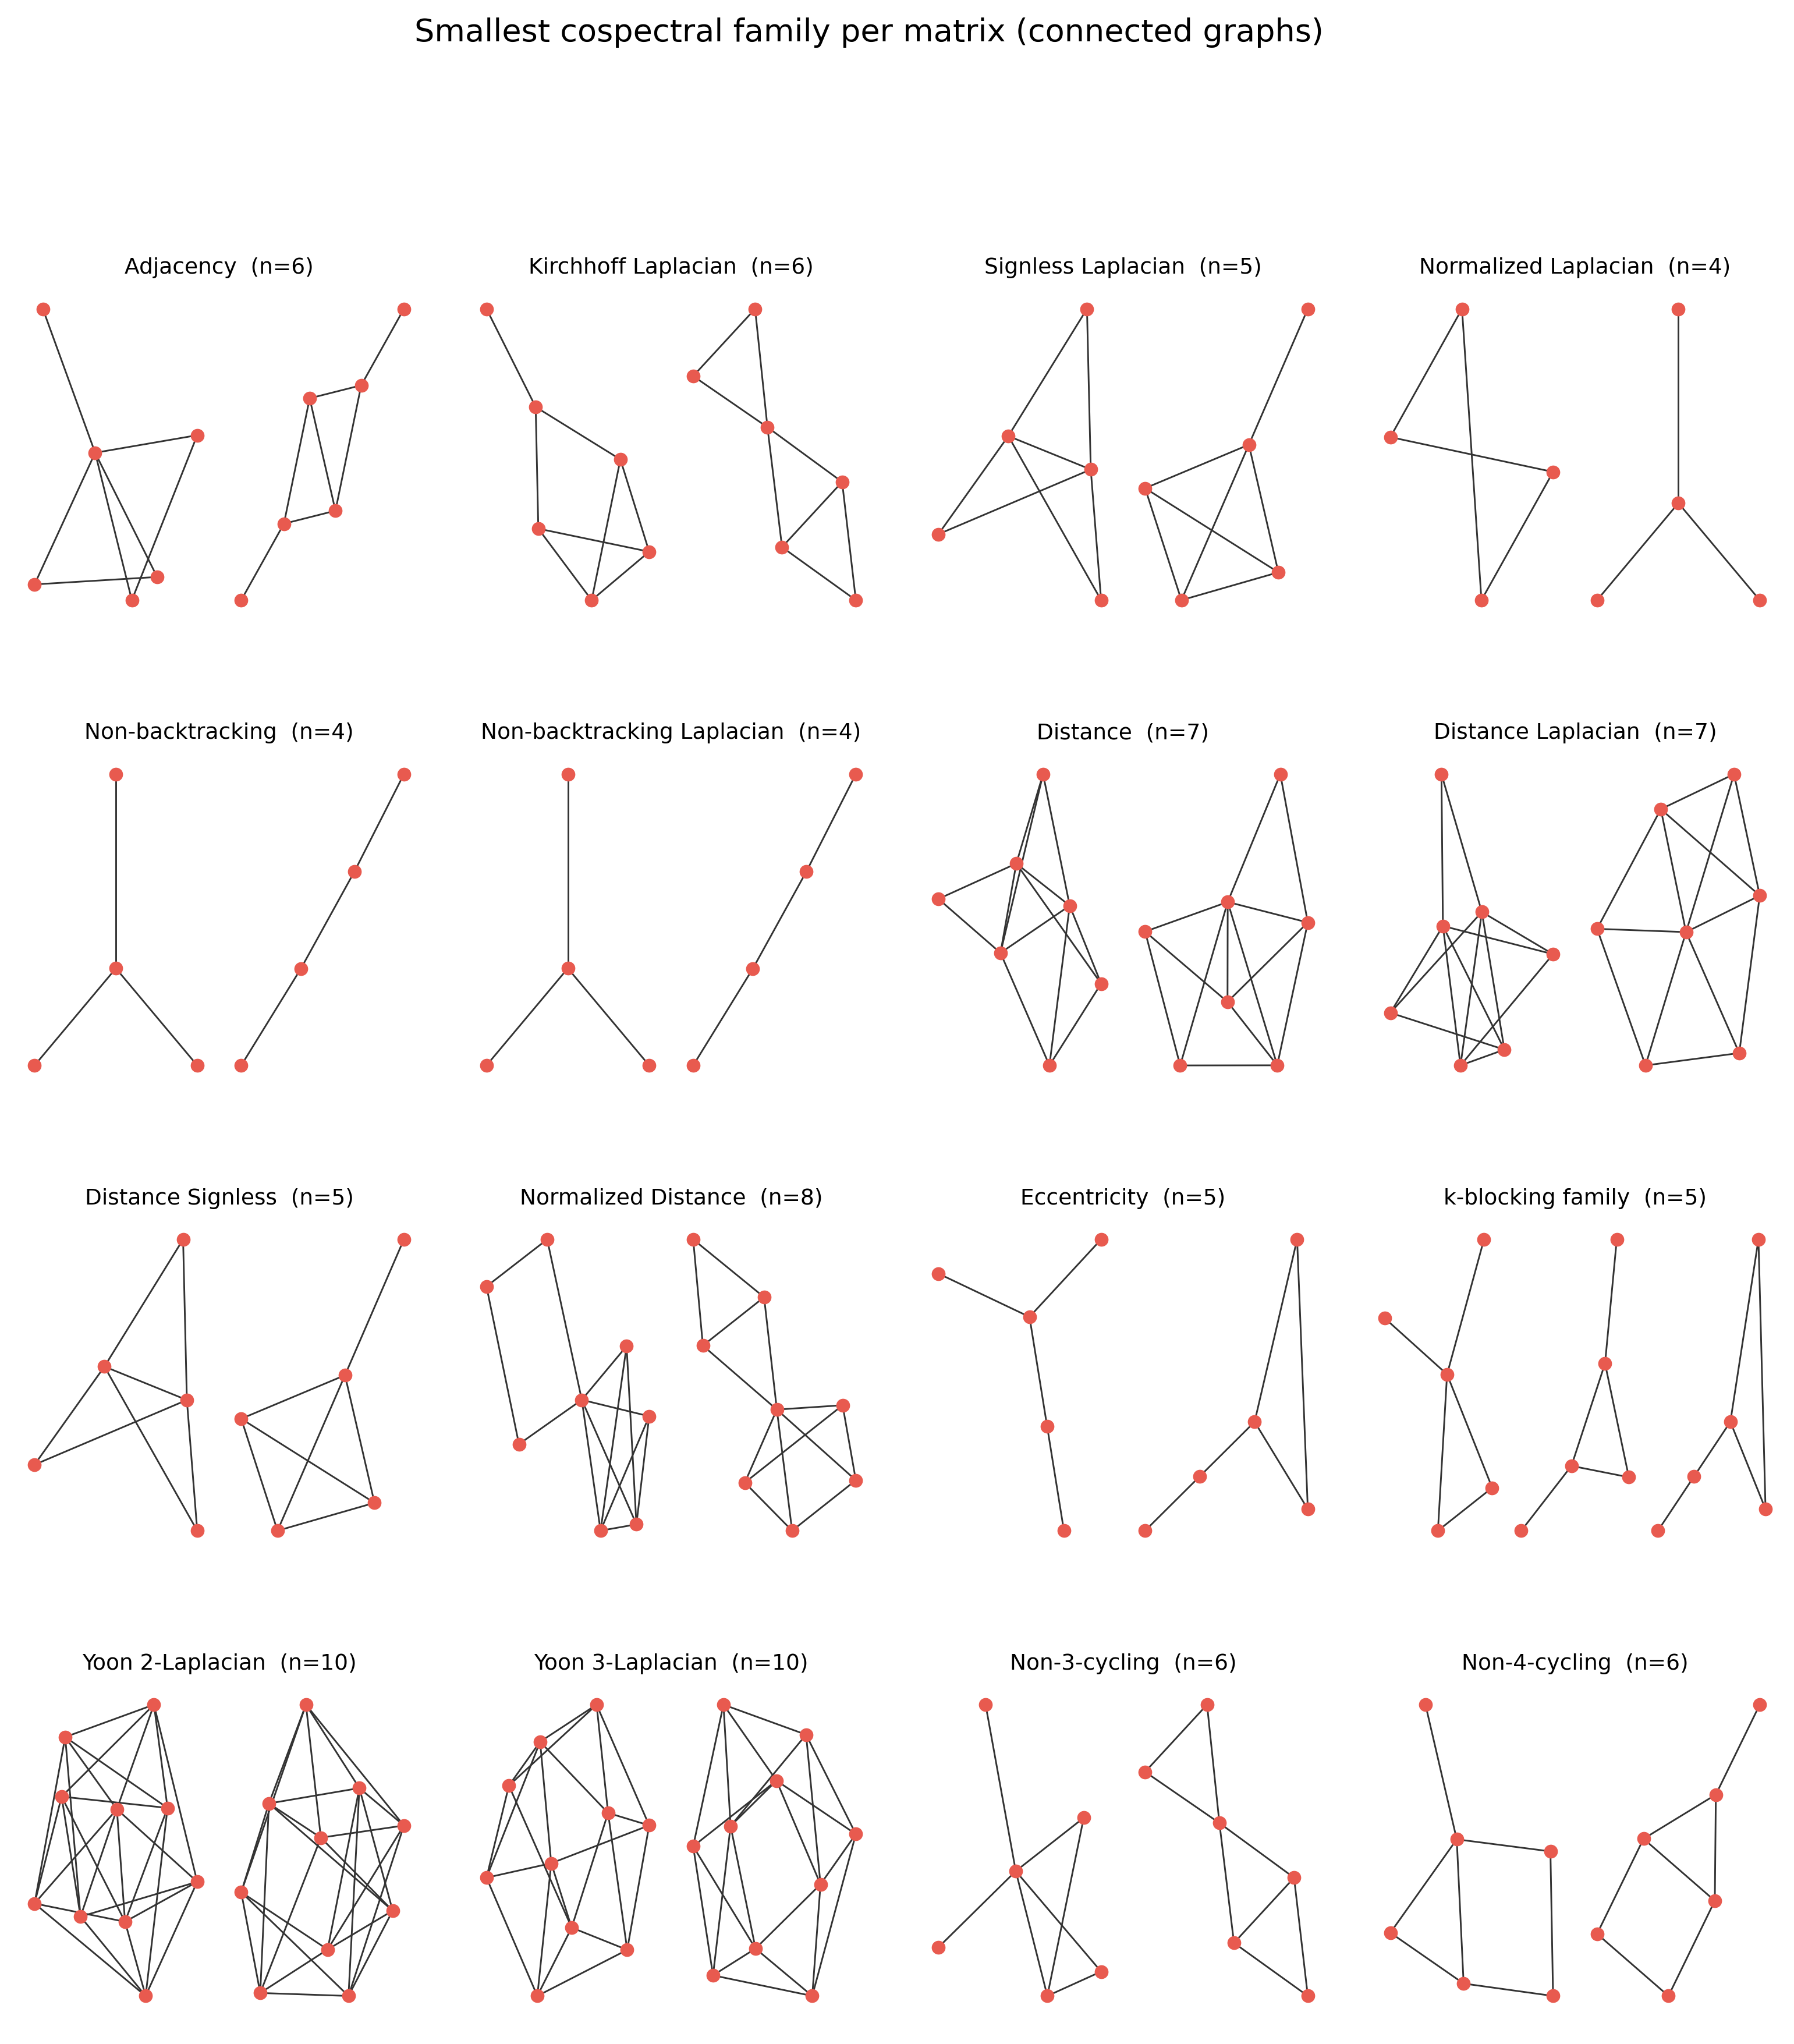
\includegraphics[keepaspectratio,alt={Figure 3.1}]{fig1_cospectral_connected.png}}
\caption{For each of the 16 matrices, the smallest cospectral family
among connected graphs (the fewest-vertex family of non-isomorphic
graphs sharing that matrix\textquotesingle s spectrum); the number of
vertices \(n\) is given per panel. The \(k\)-blocking family panel shows
a triple; all others are pairs.}\label{fig-connected}
\end{figure}

\begin{figure}
\centering
\pandocbounded{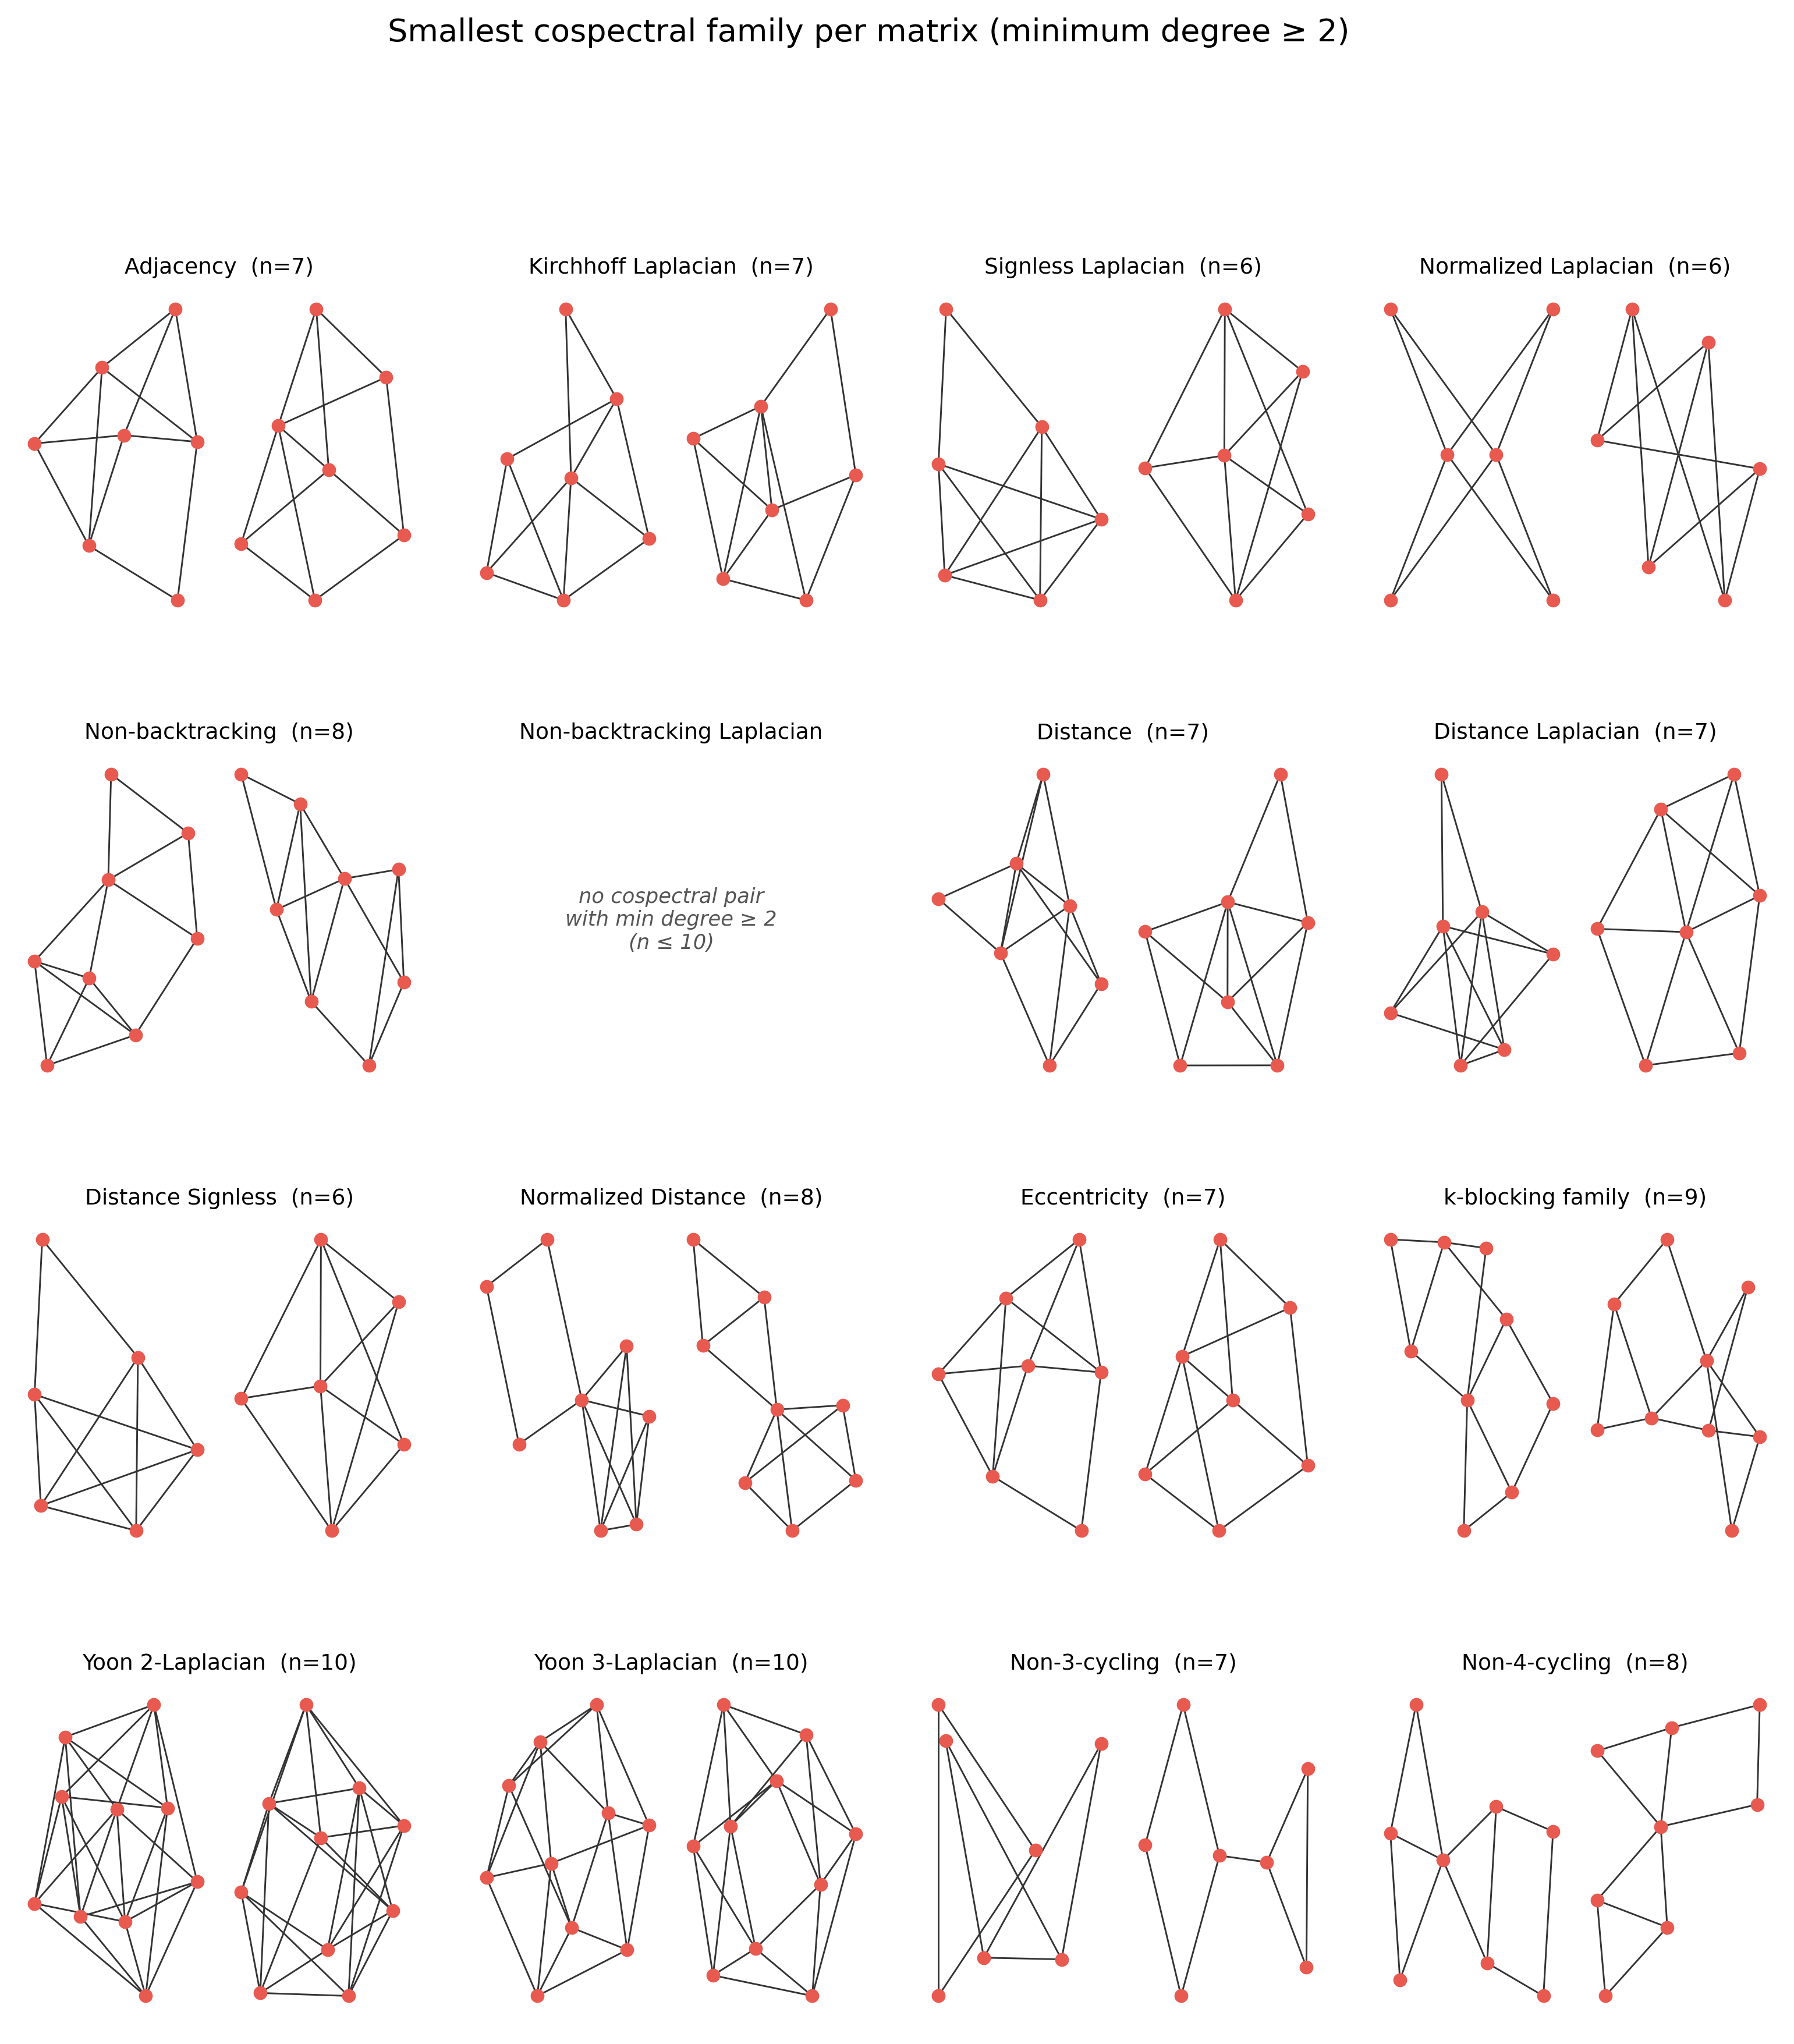
\includegraphics[keepaspectratio,alt={Figure 3.2}]{fig2_cospectral_mindeg2.png}}
\caption{The smallest cospectral family per matrix among graphs of
minimum degree at least two. The non-backtracking Laplacian has no such
family up to \(n = 10\), so every minimum-degree-\(\ge 2\) graph in the
census is determined by its non-backtracking Laplacian
spectrum.}\label{fig-mindeg2}
\end{figure}

\section{Technical Validation}\label{sec-validation}

\textbf{Reproduction of known counts.} The census sizes
(\hyperref[tbl-census]{Table 1}) match the known number of simple graphs
(OEIS A000088, {[}\hyperref[ref-oeis_a000088]{9}{]}).
SMOL\textquotesingle s count of graphs with an adjacency cospectral mate
matches OEIS A006608 (the number of graphs not determined by their
adjacency spectrum, {[}\hyperref[ref-oeis_a006608]{10}{]}) exactly
across the full range, \emph{including} \(n = 10\)
(\hyperref[tbl-oeis]{Table 3}). The combinatorial-Laplacian and
signless-Laplacian counts likewise reproduce the published
Haemers-Spence tabulations {[}\hyperref[ref-haemers2004]{5}{]}.

\begin{longtable}[]{@{}lllllll@{}}
\caption{Graphs with an adjacency cospectral mate: SMOL versus OEIS
A006608.}\label{tbl-oeis}\tabularnewline
\toprule\noalign{}
\(n\) & 5 & 6 & 7 & 8 & 9 & 10 \\
\midrule\noalign{}
\endfirsthead
\toprule\noalign{}
\(n\) & 5 & 6 & 7 & 8 & 9 & 10 \\
\midrule\noalign{}
\endhead
\bottomrule\noalign{}
\endlastfoot
SMOL (exact) & 2 & 10 & 110 & 1,722 & 51,039 & 2,560,606 \\
A006608 & 2 & 10 & 110 & 1,722 & 51,039 & 2,560,606 \\
\end{longtable}

The \(n = 10\) entry is the sharpest test, and it doubles as a
demonstration of the exactness payoff: an 8-decimal floating-point
classification gives 2,560,604 at \(n = 10\) (two short), whereas the
exact characteristic-polynomial count is 2,560,606, matching A006608.
Exactness is what makes SMOL agree with the authoritative value.

\textbf{Exactness recovers cospectral families that floating point
misses.} We compared, for each of the 13 exactly-classified matrices,
the exact characteristic-polynomial classification against an 8-decimal
floating-point eigenvalue classification. For the eleven real-spectrum
matrices the two agree exactly at \(n \le 9\); at \(n = 10\) the exact
computation recovers a small number of cospectral families that rounding
had split into singletons (\hyperref[tbl-recovered]{Table 4}), each a
pair of graphs with genuinely equal spectra wrongly separated.

The two non-backtracking matrices, whose complex spectra are exactly
where floating-point eigensolvers are least reliable, show the largest
corrections. At \(n = 10\), exact classification of the non-backtracking
matrix removes 417 spurious cospectral families that 8-decimal rounding
had created (by splitting true families inconsistently) and recovers
2,363 additional members from families rounding had split into
singletons; the non-backtracking Laplacian gains one recovered family.
We verified recovered families by independently recomputing the exact
characteristic polynomial of their members; the exact classification
never groups graphs with different characteristic polynomials, so no
spurious merges occur.

\begin{longtable}[]{@{}lll@{}}
\caption{Cospectral families among the real-spectrum matrices at
\(n = 10\) recovered by exact computation that an 8-decimal
floating-point classification splits (each recovered family is a
pair).}\label{tbl-recovered}\tabularnewline
\toprule\noalign{}
matrix & recovered families & graphs \\
\midrule\noalign{}
\endfirsthead
\toprule\noalign{}
matrix & recovered families & graphs \\
\midrule\noalign{}
\endhead
\bottomrule\noalign{}
\endlastfoot
adjacency & 1 & 2 \\
distance Laplacian & 2 & 4 \\
eccentricity & 4 & 8 \\
signless Laplacian & 1 & 2 \\
\end{longtable}

\textbf{Remaining numerical matrices.} Only the two non-\(k\)-cycling
matrices are classified numerically; their matrices reach several
thousand dimensions, beyond exact characteristic-polynomial computation
at this scale.

For the non-backtracking Laplacian, and for graphs of minimum degree at
least two, SMOL\textquotesingle s cospectral-family counts agree with
the earlier enumeration of {[}\hyperref[ref-jost2023]{7}{]}.

\section{Usage Notes}\label{sec-usage}

The database can be queried three ways: (1) directly in SQL against the
provided schema; (2) via the public REST API of the live interface
(currently at \url{https://smol-graphs-db.fly.dev}, linked from the
repository; with endpoints for single-graph lookup, filtered search,
cospectral-family listing, and on-demand spectra); (3) by loading the
per-\(n\) flat files. Eigenvalue arrays are not stored but are
recomputed on demand from \texttt{graph6} (a single function call), so
any spectrum in the dataset is reproducible bit-for-bit from the public
code.

Typical uses are looking up the cospectral mates of a given graph for
any of the 16 matrices; enumerating all cospectral families of a chosen
matrix and order to test a conjecture; or using the cospectral families
as a benchmark of spectrally-indistinguishable graphs.

\section{Code Availability}\label{sec-code}

All code to regenerate the database (enumeration, matrix construction,
exact characteristic-polynomial hashing, and the API) is openly
available at \url{https://github.com/leotrs/smol} and archived with the
dataset at Zenodo (\url{https://doi.org/10.5281/zenodo.20794132}) under
the MIT license; the dataset itself is released under CC0 1.0. The
generation pipeline is deterministic given
\texttt{nauty}\textquotesingle s \texttt{geng}, so the entire dataset is
reproducible from source.

\section{Author Contributions}\label{sec-contributions}

L.T. conceived the database, designed and implemented the generation
pipeline and the exact characteristic-polynomial cospectrality hashing,
performed all computations and validation, built the query interface,
and wrote the manuscript.

\section{Competing Interests}\label{sec-competing}

The author declares no competing interests.

\section{Funding}\label{sec-funding}

This research received no specific grant from any funding agency in the
public, commercial, or not-for-profit sectors.

\section{Acknowledgements}\label{sec-acknowledgements}

This work relies on the \texttt{nauty} package of McKay and Piperno for
graph enumeration.

\section{References}\label{references}

\begin{enumerate}
\def\labelenumi{\arabic{enumi}.}
\item
  \protect\phantomsection\label{ref-mckay2014}{}McKay, Brendan D. and Piperno, Adolfo. "Practical graph isomorphism, II". Journal of Symbolic Computation. 2014.
  \url{https://doi.org/10.1016/j.jsc.2013.09.003}
\item
  \protect\phantomsection\label{ref-brouwer2012}{}Brouwer, Andries E. and Haemers, Willem H. "Spectra of Graphs". 2012.
  \url{https://doi.org/10.1007/978-1-4614-1939-6}
\item
  \protect\phantomsection\label{ref-cvetkovic2010}{}Cvetković, Dragoš and Rowlinson, Peter and Simić, Slobodan. "An Introduction to the Theory of Graph Spectra". 2010.
  \url{https://doi.org/10.1017/CBO9780511801518}
\item
  \protect\phantomsection\label{ref-vandam2003}{}van Dam, Edwin R. and Haemers, Willem H. "Which graphs are determined by their spectrum?". Linear Algebra and its Applications. 2003.
  \url{https://doi.org/10.1016/S0024-3795(03)00483-X}
\item
  \protect\phantomsection\label{ref-haemers2004}{}Haemers, Willem H. and Spence, Edward. "Enumeration of cospectral graphs". European Journal of Combinatorics. 2004.
  \url{https://doi.org/10.1016/S0195-6698(03)00100-8}
\item
  \protect\phantomsection\label{ref-godsil1982}{}Godsil, Chris D. and McKay, Brendan D. "Constructing cospectral graphs". Aequationes Mathematicae. 1982.
  \url{https://doi.org/10.1007/BF02189621}
\item
  \protect\phantomsection\label{ref-jost2023}{}Jost, J\textbackslash"urgen and Mulas, Raffaella and Torres, Leo. "Spectral theory of the non-backtracking Laplacian for graphs". Discrete Mathematics. 2023.
  \url{https://doi.org/10.1016/j.disc.2023.113536}
\item
  \protect\phantomsection\label{ref-brinkmann2013}{}Brinkmann, Gunnar and Coolsaet, Kris and Goedgebeur, Jan and M\textbackslash\textquotesingle elot, Hadrien. "House of Graphs: a database of interesting graphs". Discrete Applied Mathematics. 2013.
  \url{https://doi.org/10.1016/j.dam.2012.07.018}
\item
  \protect\phantomsection\label{ref-oeis_a000088}{}OEIS Foundation. "Sequence A000088 (number of graphs on n unlabeled nodes)". 2024.
  \url{https://oeis.org/A000088}
\item
  \protect\phantomsection\label{ref-oeis_a006608}{}OEIS Foundation. "Sequence A006608 (number of graphs on n nodes not determined by their adjacency spectrum)". 2024.
  \url{https://oeis.org/A006608}
\item
  \protect\phantomsection\label{ref-coolsaet2023}{}Coolsaet, Kris and D\textquotesingle hondt, Sven and Goedgebeur, Jan. "House of Graphs 2.0: a database of interesting graphs and more". Discrete Applied Mathematics. 2023.
  \url{https://doi.org/10.1016/j.dam.2022.10.013}
\item
  \protect\phantomsection\label{ref-mahato2020}{}Mahato, Iswar and Gurusamy, R. and Kannan, M. Rajesh and Arockiaraj, S. "Spectra of eccentricity matrices of graphs". Discrete Applied Mathematics. 2020.
  \url{https://doi.org/10.1016/j.dam.2020.06.004}
\item
  \protect\phantomsection\label{ref-yoon2025}{}Yoon, Mary. "Graph Laplacians with higher accuracy". arXiv preprint arXiv:2504.04461. 2025.
  \url{https://arxiv.org/abs/2504.04461}
\item
  \protect\phantomsection\label{ref-arrigo2020}{}Arrigo, Francesca and Higham, Desmond J. and Noferini, Vanni. "Beyond non-backtracking: non-cycling network centrality measures". Proceedings of the Royal Society A. 2020.
  \url{https://doi.org/10.1098/rspa.2019.0653}
\end{enumerate}

\end{document}
